
\documentclass{beamer}
\usecolortheme{dove}
\setbeamertemplate{navigation symbols}{}
\usepackage{amsmath,amssymb,amsfonts,amsthm, multicol, subfigure, color}
\usepackage{bm}
\usepackage{graphicx}
\usepackage{tabularx}
\usepackage{booktabs}
\usepackage{hyperref}
\usepackage{pdfpages}
\usepackage{xcolor}
\definecolor{seagreen}{RGB}{46, 139, 87}
\def\independenT#1#2{\mathrel{\rlap{$#1#2$}\mkern2mu{#1#2}}}
\newcommand\indep{\protect\mathpalette{\protect\independenT}{\perp}}
\def\log{\text{log}}
\newcommand\logit{\text{logit}}
\newcommand\iid{\stackrel{\text{iid}}{\sim}}
\newcommand\E{\text{E}}
\newcommand\V{\text{V}}
\renewcommand\P{\text{P}}
\newcommand{\Cov}{\text{Cov}}
\newcommand{\Cor}{\text{Cor}}
\newcommand\doop{\texttt{do}}
\usepackage{stackrel}
\usepackage{tikz}
\usetikzlibrary{arrows,shapes.arrows,positioning,shapes,patterns,calc}
\newcommand\slideref[1]{\vskip .1cm \tiny \textcolor{gray}{{#1}}}
\newcommand\red[1]{\color{red}#1}
\newcommand\blue[1]{\color{blue}#1}
\newcommand\gray[1]{\color{gray}#1}
\newcommand\seagreen[1]{\color{seagreen}#1}
\newcommand\purple[1]{\color{purple}#1}
\newcommand\orange[1]{\color{orange}#1}
\newcommand\black[1]{\color{black}#1}
\newcommand\white[1]{\color{white}#1}
\newcommand\teal[1]{\color{teal}#1}
\newcommand\magenta[1]{\color{magenta}#1}
\newcommand\Fuchsia[1]{\color{Fuchsia}#1}
\newcommand\BlueGreen[1]{\color{BlueGreen}#1}
\newcommand\bblue[1]{\textcolor{blue}{\textbf{#1}}}
\newcommand\bred[1]{\textcolor{red}{\textbf{#1}}}
\newcommand\bgray[1]{\textcolor{gray}{\textbf{#1}}}
\newcommand\bgreen[1]{\textcolor{seagreen}{\textbf{#1}}}
\newcommand\bref[2]{\href{#1}{\color{blue}{#2}}}
\colorlet{lightgray}{gray!40}
\pgfdeclarelayer{bg}    % declare background layer for tikz
\pgfsetlayers{bg,main} % order layers for tikz
\newcommand\mycite[1]{\begin{scriptsize}\textcolor{darkgray}{(#1)}\end{scriptsize}}
\newcommand{\tcframe}{\frame{
%\small{
\only<1|handout:0>{\tableofcontents}
\only<2|handout:1>{\tableofcontents[currentsubsection]}}
%}
}

\usepackage[round]{natbib}
\bibliographystyle{humannat-mod}
\setbeamertemplate{enumerate items}[default]
\usepackage{mathtools}

\newcommand{\goalsframe}{\begin{frame}{Learning goals for today}
At the end of class, you will be able to:
\begin{enumerate}
\item Trace inverse probability weighting to survey sampling
\item Apply the Horvitz-Thompson estimator for causal inference
\item Recognize the bias-variance tradeoff of trimmed weights
\item Estimate the ATE, ATT, and ATC by weighting
%\item Next time: Assume structure on potential outcomes with a marginal structural model
\end{enumerate} \vskip .2in
\end{frame}}

\title{13. Inverse Probability Weighting}
\author{Ian Lundberg\\Cornell Info 6751: Causal Inference in Observational Settings\\Fall 2022}
\date{4 Oct 2022}

\begin{document}

\maketitle

\goalsframe

\begin{frame}{Inverse probability weighting: Sampling} \pause
\begin{tikzpicture}[x = \textwidth, y = .8\textheight]
\node at (0,0) {};
\node at (1,1) {};
\node[anchor = north] at (.45,.9) {$L = 0$};
\node[anchor = north] at (.85,.9) {$L = 1$};
\draw[rounded corners] (.3,.4) rectangle (.6,1);
\draw[rounded corners] (.7,.4) rectangle (1,1);
\node<3->[anchor = north west, gray, font = \Huge] (unsamp) at (0,.9) {$\bullet$};
\node<3->[anchor = west, gray] at (unsamp.east) {Unsampled};
\node<3->[anchor = north west, blue, font = \Huge] (samp) at (unsamp.south west) {$\bullet$};
\node<3->[anchor = west, blue] (samp.east) at (samp.east) {Sampled};
% L = 0
\node[gray, font = \Huge] at (.4,.6) {$\bullet$};
\node<1-3>[gray, font = \Huge] at (.5,.5) {$\bullet$};
\node<4->[blue, font = \Huge] at (.5,.5) {$\bullet$};
\node[gray, font = \Huge] at (.55,.45) {$\bullet$};
\node[gray, font = \Huge] at (.45,.7) {$\bullet$};
% L = 1
\onslide<1-4>{
\node[gray, font = \Huge] at (.75,.52) {$\bullet$};
\node[gray, font = \Huge] at (.85,.44) {$\bullet$};
\node[gray, font = \Huge] at (.95,.63) {$\bullet$};
}
\onslide<5->{
\node[blue, font = \Huge] at (.75,.52) {$\bullet$};
\node[blue, font = \Huge] at (.85,.44) {$\bullet$};
\node[blue, font = \Huge] at (.95,.63) {$\bullet$};
}
\node[gray, font = \Huge] at (.9,.72) {$\bullet$};
% P(S)
\node<6-> at (.45, .2) {$\begin{aligned}\pi_i &= \P(S = 1\mid L_i = 0)\\&= \frac{1}{4}\\\onslide<7->{w_i&=\frac{1}{\pi_i}=4}\end{aligned}$};
\node<6-> at (.85, .2) {$\begin{aligned}\pi_i &= \P(S = 1\mid L_i = 1)\\&= \frac{3}{4}\\\onslide<7->{w_i &=\frac{1}{\pi_i}= \frac{4}{3}}\end{aligned}$};
\node<7->[anchor = west] at (0,.1) {Each counts for:};
\end{tikzpicture}
\end{frame}

\begin{frame}
The Horvitz-Thompson estimator for a population mean:
$$\hat\E(Y) = \frac{1}{N} \sum_{i:S_i=1} \frac{Y_i}{\pi_i}$$
where $N$ is the population size and\\$\pi_i$ is the known probability of sampling
\end{frame}

\begin{frame}{Inverse probability weighting: Conditional randomizaton} \pause


\begin{tikzpicture}[x = \textwidth, y = .8\textheight]
\node at (0,0) {};
\node at (1,1) {};
\node[anchor = north] at (.45,.9) {$L = 0$};
\node[anchor = north] at (.85,.9) {$L = 1$};
\draw[rounded corners] (.3,.4) rectangle (.6,1);
\draw[rounded corners] (.7,.4) rectangle (1,1);
\node<3->[anchor = north west, gray, font = \Huge] (unsamp) at (0,.9) {$\bullet$};
\node<3->[anchor = west, gray] at (unsamp.east) {Untreated};
\node<3->[anchor = north west, blue, font = \Huge] (samp) at (unsamp.south west) {$\bullet$};
\node<3->[anchor = west, blue] (samp.east) at (samp.east) {Treated};
% L = 0
\node[gray, font = \Huge] at (.4,.6) {$\bullet$};
\node<1-3>[gray, font = \Huge] at (.5,.5) {$\bullet$};
\node<4->[blue, font = \Huge] at (.5,.5) {$\bullet$};
\node[gray, font = \Huge] at (.55,.45) {$\bullet$};
\node[gray, font = \Huge] at (.45,.7) {$\bullet$};
% L = 1
\onslide<1-4>{
\node[gray, font = \Huge] at (.75,.52) {$\bullet$};
\node[gray, font = \Huge] at (.85,.44) {$\bullet$};
\node[gray, font = \Huge] at (.95,.63) {$\bullet$};
}
\onslide<5->{
\node[blue, font = \Huge] at (.75,.52) {$\bullet$};
\node[blue, font = \Huge] at (.85,.44) {$\bullet$};
\node[blue, font = \Huge] at (.95,.63) {$\bullet$};
}
\node[gray, font = \Huge] at (.9,.72) {$\bullet$};
% P(S)
\node<6->[anchor = west] at (0,.3) {$\pi_i = \P(A_i\mid L_i) = $};
\node<6->[anchor = west] at (.3,.3) {$\begin{cases}\frac{1}{4}&\text{if }A_i = 1\\\frac{3}{4}&\text{if }A_i = 0\end{cases}$};
\node<7->[anchor = west] at (.7,.3) {$\begin{cases}\frac{3}{4}&\text{if }A_i = 1\\\frac{1}{4}&\text{if }A_i = 0\end{cases}$};
\node<8->[anchor = west] at (0,.1) {Each counts for:};
\node<9->[anchor = west] at (.3,.1) {$\begin{cases}\frac{4}{1}&\text{if }A_i = 1\\\frac{4}{3}&\text{if }A_i = 0\end{cases}$};
\node<10->[anchor = west] at (.7,.1) {$\begin{cases}\frac{4}{3}&\text{if }A_i = 1\\\frac{4}{1}&\text{if }A_i = 0\end{cases}$};
\end{tikzpicture}

\end{frame}

\begin{frame}

Inverse probability weighted (IPW) estimator\\for the average treatment effect (ATE)
$$\E(Y^1) - \E(Y^0) = \frac{1}{N}\sum_{i:A_i=1}\frac{Y_i}{\pi_i} - \frac{1}{N}\sum_{i:A_i=0}\frac{Y_i}{\pi_i}$$
where $\pi_i = \P(A = a_i\mid \vec{L} = \vec{\ell}_i)$\\
is the probability of the observed treatment given confounders

\end{frame}

\begin{frame}{Inverse probability weighting: Mathematical proof\footnote{Hern\'an \& Robins Technical Point 2.3}} \pause

\begin{small}
\begin{align}
&\E\left(\frac{\mathbb{I}(A = a)}{\P(A = a\mid \vec{L})}Y\right) \\
\onslide<3->{
&= \E\left(\frac{\mathbb{I}(A = a)}{\P(A = a\mid \vec{L})}Y^a\right) &\text{consistency} \\
}
\onslide<4->{
&= \E\left(\E\left[\frac{\mathbb{I}(A = a)}{\P(A = a\mid \vec{L})}Y^a\mid \vec{L}\right]\right) &\text{iterated expectation} \\
}
\onslide<5->{
&= \E\left(\E\left[\frac{\mathbb{I}(A = a)}{\P(A = a\mid \vec{L})}\mid\vec{L}\right]\E\left[Y^a\mid \vec{L}\right]\right) &\text{exchangeability} \\
}
\onslide<6->{
&= \E\left(\E\left[Y^a\mid \vec{L}\right]\right) &\text{since left term was 1} \\
}
&= \E(Y^a) &\onslide<7->{\text{iterated expectation}}
\end{align}
\end{small}

\end{frame}

\begin{frame}{Inverse probability weighting: Observational studies}

In an experiment, we control treatment assignment. \\
We know the dashed edge does not exist. \\
We know the propensity score $\pi$. \\
\begin{center}
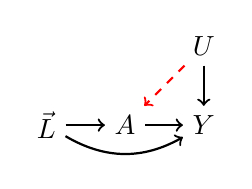
\begin{tikzpicture}
\node (l) at (0,0) {$\vec{L}$};
\node (a) at (1,0) {$A$};
\node (y) at (2,0) {$Y$};
\node (u) at (2,1) {$U$};
\draw[->, thick] (l) -- (a);
\draw[->, thick] (a) -- (y);
\draw[->, thick] (l) to[bend right] (y);
\draw[->, thick, red, dashed] (u) -- (a);
\draw[->, thick] (u) -- (y);
\end{tikzpicture}
\end{center} \pause
In an observational study, we do not control assignment.\\ \pause
We assume the dashed edge does not exist.\\ \pause
We estimate the propensity score. \vskip .2in \pause
Otherwise all estimators (including IPW) are the same.

\end{frame}

\begin{frame}{Inverse probability weighting: Nonparametric procedure}

\pause
\begin{enumerate}[<+->]
\item Assume a DAG where $\vec{L}$ blocks backdoor paths
\item Stratify the by $\vec{L}$
\item Empirically estimate $\hat\pi_i$ as the proportion with $A = a_i$ within the stratum $\vec{L} = \vec\ell_i$ of unit $i$
\item Apply the IPW estimator
\end{enumerate} \vskip .2in
\onslide<5->{$$\hat\E(Y^a) = \frac{1}{N}\sum_{i:A_i=a}\frac{Y_i}{\hat\pi_i}$$}

\end{frame}

\begin{frame}{Inverse probability weighting: Parametric procedure\footnote{On the Hajek estimator, see Hern\'an \& Robins Technical Point 12.1}}

\pause
\begin{enumerate}[<+->]
\item Assume a DAG where $\vec{L}$ blocks backdoor paths
\item Estimate the propensity score $\hat\pi_i$ with a model
$$\begin{aligned}
\hat\P(A = 1\mid \vec{L}) &= \logit^{-1}\left(\hat\alpha + \hat{\vec\gamma}\vec{L}\right) \\
\hat\pi_i &= \begin{cases}
\logit^{-1}\left(\hat\alpha + \hat{\vec\gamma}\vec{L}\right) &\text{if }A_i=1 \\
1 - \logit^{-1}\left(\hat\alpha + \hat{\vec\gamma}\vec{L}\right) &\text{if }A_i=0 \\
\end{cases}
\end{aligned}$$
\item Apply an IPW estimator
\end{enumerate} \vskip .2in
\onslide<5->{
$$\begin{aligned}
\hat\E(Y^a) &= \frac{1}{N}\sum_{i:A_i=a}\frac{Y_i}{\hat\pi_i} &\text{(Horvitz-Thompson)} \\
&\text{or} \\
\hat\E(Y^a) &= \frac{1}{\sum_{i:A_i=a}\frac{1}{\hat\pi_i}}\sum_{i:A_i=a}\frac{Y_i}{\hat\pi_i} &\text{(Hajek)}
\end{aligned}$$
}

\end{frame}

\begin{frame}{Problem: Extreme weights create high variance}

\pause
Suppose a stratum $\vec{L} = \vec\ell$ contains
\begin{itemize}
\item 100 untreated units
\item 1 treated unit
\end{itemize} \pause
The treated unit gets a weight of 100.\vskip .2in \pause
The estimate depends heavily on which treated unit happens to be included in the sample $\rightarrow$ high-variance estimator \vskip .2in \pause
Two solutions
\begin{enumerate}
\item Trim the weights
\item Truncate the weights
\end{enumerate} \pause
Both solutions accept bias in order to reduce variance

\end{frame}

\begin{frame}{Accepting bias to reduce variance: Trimming}

\begin{tikzpicture}[x = \textwidth, y = .8\textheight]
\node at (0,0) {};
\node at (1,1) {};
\node<1>[anchor = west] at (0,.5) {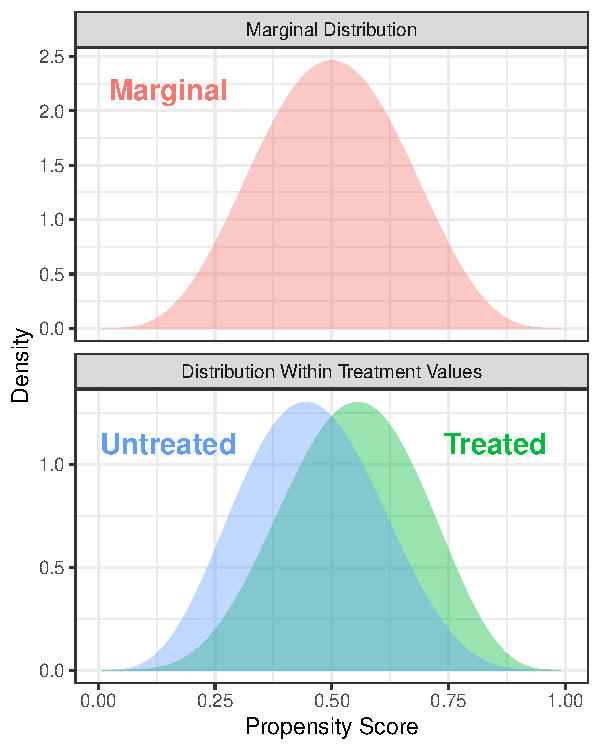
\includegraphics[height = .8\textheight]{figures/propensity_overlap}};
\node<2-3>[anchor = west] at (0,.5) {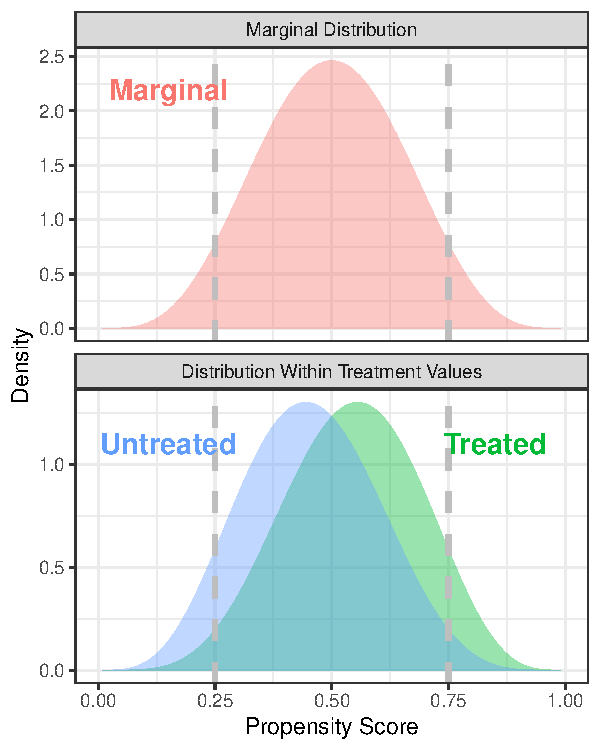
\includegraphics[height = .8\textheight]{figures/propensity_overlap_1}};
\node<3->[anchor = west, align = left] at (.6,.7) {Drop units with\\extreme weights};
\node<4->[anchor = west] at (0,.5) {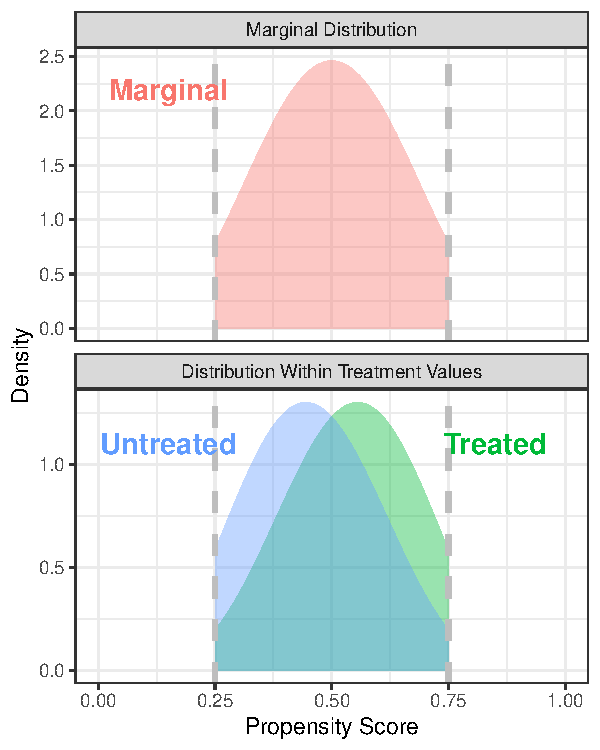
\includegraphics[height = .8\textheight]{figures/propensity_overlap_trim}};
\node<5->[anchor = west, align = left] at (.6,.5) {Changes target population\\--- Biased for full population};
\end{tikzpicture}

\end{frame}

\begin{frame}{Accepting bias to reduce variance: Weight truncation}

\begin{tikzpicture}[x = \textwidth, y = .8\textheight]
\node at (0,0) {};
\node at (1,1) {};
\node<1-2>[anchor = west] at (0,.5) {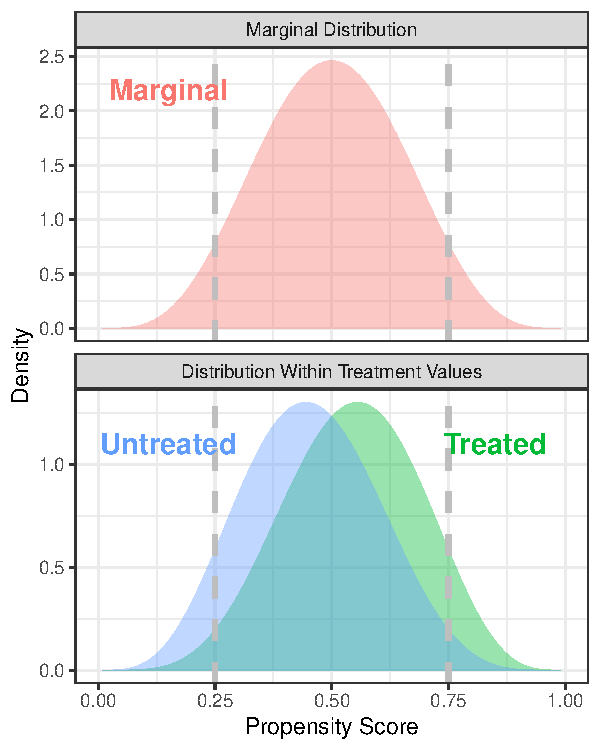
\includegraphics[height = .8\textheight]{figures/propensity_overlap_1}};
\node<2->[anchor = west, align = left] at (.6,.7) {Truncate values of\\extreme weights};
\node<3->[anchor = west] at (0,.5) {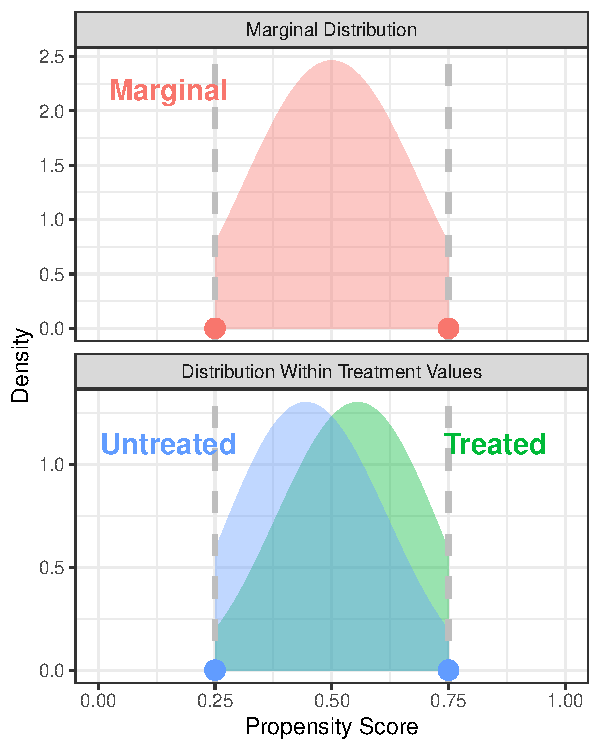
\includegraphics[height = .8\textheight]{figures/propensity_overlap_truncate}};
\node<4->[anchor = west, align = left] at (.6,.5) {Biased: Ignores\\some confounding};
\end{tikzpicture}

\end{frame}

\begin{frame}{Weighting for the ATE, ATT, ATC} \pause


\begin{tikzpicture}[x = \textwidth, y = .8\textheight]
\node at (0,0) {};
\node at (1,1) {};
\node[anchor = north] at (.45,.9) {$L = 0$};
\node[anchor = north] at (.85,.9) {$L = 1$};
\draw[rounded corners] (.3,.4) rectangle (.6,1);
\draw[rounded corners] (.7,.4) rectangle (1,1);
\node[anchor = north west, gray, font = \Huge] (unsamp) at (0,.9) {$\bullet$};
\node[anchor = west, gray] at (unsamp.east) {Untreated};
\node[anchor = north west, blue, font = \Huge] (samp) at (unsamp.south west) {$\bullet$};
\node[anchor = west, blue] (samp.east) at (samp.east) {Treated};
% L = 0
\node[gray, font = \Huge] at (.4,.6) {$\bullet$};
\node[blue, font = \Huge] at (.5,.5) {$\bullet$};
\node[gray, font = \Huge] at (.55,.45) {$\bullet$};
\node[gray, font = \Huge] at (.45,.7) {$\bullet$};
% L = 1
\node[blue, font = \Huge] at (.75,.52) {$\bullet$};
\node[blue, font = \Huge] at (.85,.44) {$\bullet$};
\node[blue, font = \Huge] at (.95,.63) {$\bullet$};
\node[gray, font = \Huge] at (.9,.72) {$\bullet$};
% ATE weights
\node<3-7>[anchor = north west, align = left] at (0,.3) {For ATE:\\$w_i = \frac{1}{\P(A = a_i\mid L = \ell_i)}$};
\node<4-7>[anchor = north, align = left, gray, font = {\bf\huge}] at (.45,.35) {$\frac{1}{3/4} = \frac{4}{3}$};
\node<5-7>[anchor = north, align = left, blue, font = {\bf\huge}] at (.45,.15) {$\frac{1}{1/4} = \frac{4}{1}$};
\node<6-7>[anchor = north, align = left, gray, font = {\bf\huge}] at (.85,.35) {$\frac{1}{1/4} = \frac{4}{1}$};
\node<7>[anchor = north, align = left, blue, font = {\bf\huge}] at (.85,.15) {$\frac{1}{3/4} = \frac{4}{3}$};
% ATT weights
\node<8-12>[anchor = north west, align = left] at (0,.3) {For ATT?};
\node<13-14>[anchor = north west, align = left] at (0,.3) {For ATT:\\$w_i = \frac{\P(A = 1\mid L = \ell_i)}{\P(A = a_i\mid L = \ell_i)}$};
\node<10-13>[anchor = east, align = left, blue, font = {\bf\huge}] at (.55,.1) {$1$};
\node<12-13>[anchor = east, align = left, blue, font = {\bf\huge}] at (.95,.1) {$1$};
\node<9-13>[anchor = east, align = left, gray, font = {\bf\huge}] at (.55,.3) {$\frac{1}{3}$};
\node<11-13>[anchor = east, align = left, gray, font = {\bf\huge}] at (.95,.3) {$\frac{3}{1}$};
\node<14>[anchor = east, align = left, blue, font = {\bf\huge}] at (.55,.1) {$\frac{1/4}{1/4} = 1$};
\node<14>[anchor = east, align = left, blue, font = {\bf\huge}] at (.95,.1) {$\frac{3/4}{3/4} = 1$};
\node<14>[anchor = east, align = left, gray, font = {\bf\huge}] at (.55,.3) {$\frac{1/4}{3/4} = \frac{1}{3}$};
\node<14>[anchor = east, align = left, gray, font = {\bf\huge}] at (.95,.3) {$\frac{3/4}{1/4} = \frac{3}{1}$};
% ATC weights
\node<15->[anchor = north west, align = left] at (0,.3) {For ATC:\\$w_i = \frac{\P(A = 0\mid L = \ell_i)}{\P(A = a_i\mid L = \ell_i)}$};
\node<16->[anchor = east, align = left, gray, font = {\bf\huge}] at (.55,.3) {$\frac{3/4}{3/4} = 1$};
\node<17->[anchor = east, align = left, blue, font = {\bf\huge}] at (.55,.1) {$\frac{3/4}{1/4} = 3$};
\node<18->[anchor = east, align = left, gray, font = {\bf\huge}] at (.95,.3) {$\frac{1/4}{1/4} = 1$};
\node<19->[anchor = east, align = left, blue, font = {\bf\huge}] at (.95,.1) {$\frac{1/4}{3/4} = \frac{1}{3}$};
\end{tikzpicture}

\end{frame}

\begin{frame}{Weighting for the ATE, ATT, ATC}

General formula:
$$
w_i = \frac{\text{Size of target population in }\vec{L} = \vec\ell_i}{\text{Size of factual population in }\vec{L} = \vec\ell_i}
$$ \vskip .2in
Intuition:
\begin{itemize}
\item Normalize the factual population across strata \hfill (denominator)
\item Upweight to the counterfactual population \hfill (numerator)
\end{itemize}

\end{frame}

\begin{frame}{Inverse probability weighting: Reading}

Hern\'an \& Robins
\begin{itemize}
\item 2.4
\item 12.1--12.3
\end{itemize}

\end{frame}

\goalsframe

\begin{frame}{Let me know what you are thinking}

\begin{huge} \bref{https://tinyurl.com/CausalQuestions}{tinyurl.com/CausalQuestions} \end{huge}
\vskip .7in

Office hours TTh 11am-12pm and at \bref{https://calendly.com/ianlundberg/office-hours}{calendly.com/ianlundberg/office-hours}\\Come say hi!

\end{frame}

\end{document}

